\documentclass{standalone}
\usepackage{tikz}
\usepackage{ctex,siunitx}
\setCJKmainfont{Noto Serif CJK SC}
\usepackage{tkz-euclide}
\usepackage{amsmath}
\usetikzlibrary{patterns, calc}
\usetikzlibrary {decorations.pathmorphing, decorations.pathreplacing, decorations.shapes,}

\begin{document}
\small
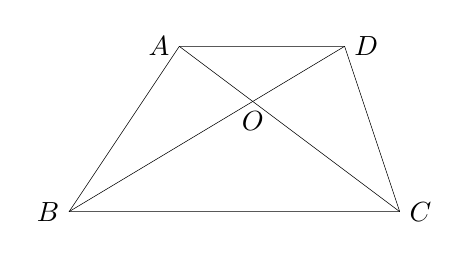
\begin{tikzpicture}[>=stealth,scale=0.7]
  \tkzSetUpPoint[fill=black]
  % \useasboundingbox(-1,-0.75)rectangle(3.7,1.4);
  \tkzDefPoints{0/0/B, 6/0/C, 5/3/D, 2/3/A}
  \tkzInterLL(A,C)(B,D)\tkzGetPoint{O}
  \tkzDrawPolygon(A,B,C,D)
  \tkzDrawSegments(A,C B,D)
  \tkzLabelPoints[left](A,B)
  \tkzLabelPoints[right](C,D)
  \tkzLabelPoints[below](O)
\end{tikzpicture}
\end{document}